%!TEX root = ../../../report.tex

\subsection{Dataflow}

When designing an energy efficient system, dataflow is of great importance. The
software on the MCU has been designed to minimize the number of data stores and
movements, and CPU usage is kept to a minimum so that the processor can be
turned off to save energy. \todo[inline]{It seems natural to mention something
more about the different GG energy modes here, or somewhere close - maybe a new
subsection? This has also been mentioned earlier in software architecture, so
take a look there and see if that can be moved up here. -JK}

\subsubsection{Peripherals}
The MCU facilitates audio I/O from ADC, DAC, SDCard and serial port interface to
and from the FPGA.
\todo{is serial audio I/O implemented?}
\begin{figure}[h]
	\centering
	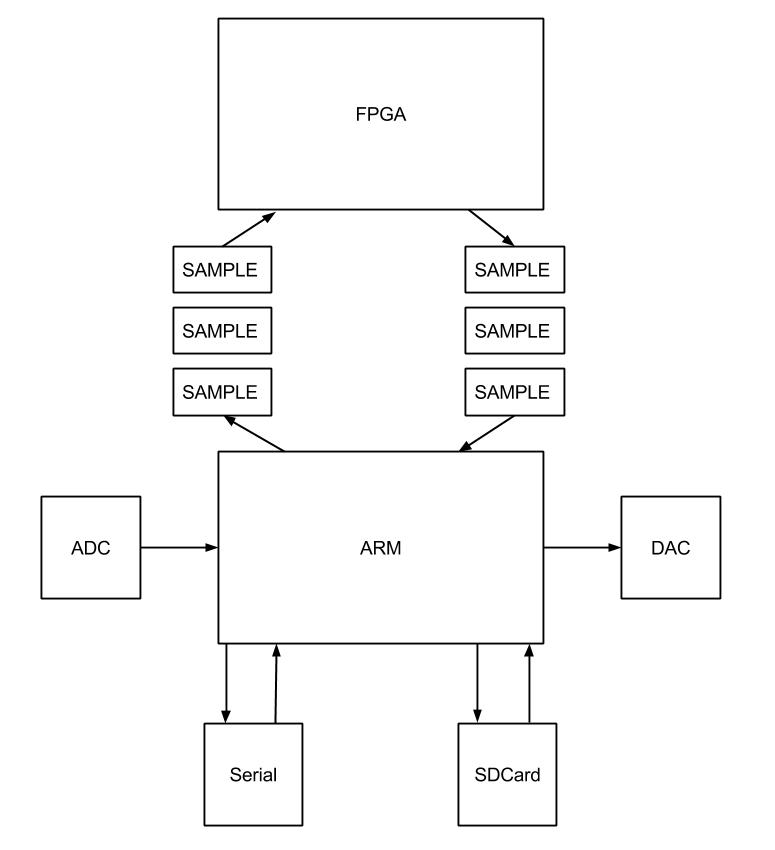
\includegraphics[height=150px]{figures/sw/sample-flow.png}
	%\begin{tikzpicture}[shorten >= 1pt, node distance=3cm, on grid, auto]
	%	\node[draw,rectangle,minimum size=2cm] (fpga) {FPGA};
	%	\node[draw,rectangle,below of=fpga,minimum size=2cm] (arm) {ARM};
	%\end{tikzpicture}
	\caption{Flow of samples}
	\label{fig:sw_sample_flow}
\end{figure}
\todo{Tikzify}


\todo[inline]{explain the figure and refer to it in the text -JK}

\subsubsection{External Bus Interface}
The MCU is connected to the FPGA and SRAM through the EBI. This leads to a
simple interface with these units since the EBI is memory mapped on the MCU.
Communicating with the FPGA is done by reading and writing to memory.

\todo{more about how the bus is implemented on the MCU}

\subsubsection{Direct Memory Access} DMA provides the ability to move data
without the intervention of the CPU. This is used extensively to implement the
dataflow when the MCU is in a low energy mode. The CPU is only used to configure
and refresh the DMA channels in between transfers. The MCU provides 12
independent DMA channels which can move data between peripherals, RAM, Flash and
the EBI.

The main path of dataflow goes from RAM on the MCU to the internal buffers in
the FPGA, and back again to RAM in the MCU. This dataflow path utilizes four DMA
channels.

\missingfigure{Figure showing RAM => FPGA => RAM}

In addition, a DMA is assigned for each ADC and DAC whenever they are used as
input and output, respectively. When SDCard is used, the contents of the files
are read and written directly to and from RAM by the CPU.

\paragraph{Deinterleaving of Samples}
When reading from both a WAV file and the ADC, samples from the stereo channels
are interleaved. The FPGA handles as mentioned each channel in each its own
audio pipeline. On the input side the samples need to de-interleaved and on
output they are interleaved again. This is why two DMA channels are needed for
the input, and two are needed for the output. A complementary version of this
procedure is implemented on the CPU and power comparison plots which are
included in the results chapter. \todo{Make sure they are. Rewrite for better flow - JK}

\missingfigure{Figure showing deinterleaving and interleaving}

The samples are de-interleaved by letting two DMA channels read from the same
source and write to the correct pipeline for the correct channel. The first DMA
copies the samples for the left stero channel, and start without a offset. The
second DMA copies the samples for the right stereo channel and start with an
offset of one sample. Both DMAs read only every second sample and writes them
continuously to the FPGA input buffers.

The interleaving process on output side works in the same way. The DMA reading
from the pipeline containing the left stereo channel samples writes to the
memory without a starting offset. The right channel DMA writes with an offset by
one sample.
\todo[inline]{Rewrite for better flow - JK}

\paragraph{Triggering Transfers}

All the DMA transfers are triggered by the use of one clock, the sample clock.
This clock is run at the sample speed 11 kilohertz when using the DAC or ADC. Or
an arbitrary frequency when sampling from SD to SD. The clock signal is fed into
the Peripheral Reflex System (PRS) of the MCU and propagates through the system
using the following scheme

%\newpage %re-insert if figure breaks across pages
\begin{verbatim}

                        | Audio in
                        V
+------+  +-----+    +------+   +-----+     +--------+
|TIMER0|->| PRS |-+->| ADC0 |-->| DMA |---->| Buffer |
+------+  +-----+ |  +------+   +-----+     +--------+
                  |     .                      / \
                  |     .                     /   \
                  |     .                    V     V
                  |     .              +-----+     +-----+
                  |     +....irq......>| DMA |....>| DMA |
                  |                    +-----+     +-----+
                  |                       |           |
                  |                       V           V
                  |                   +------+    +-------+
                  |                   | FPGA |    | FPGA  |
                  |                   | Left |    | Right |
                  |                   +------+    +-------+
                  |                       |           |
                  |                       V           V
                  |                    +-----+     +-----+
                  |     +....irq......>| DMA |....>| DMA |
                  |     .              +-----+     +-----+
                  |     .                    \     /
                  |     .                     \   /
                  |     .                       V
                  |  +------+   +-----+     +--------+
                  +->| DAC0 |<--| DMA |<----| Buffer |
                     +------+   +-----+     +--------+
                        |
                        V Audio out
\end{verbatim}

Here, both the DAC and ADC consumes the PRS signal originated from TIMER0. The
DMA copying from the ADC to the RAM buffer, and the two DMAs performing the
de-interleaving of the input samples, receive a pulse each time the ADC has
buffered $N$ samples. They then perform a sequence of copy actions resulting
in the input samples ending up inside the pipeline buffers of the FPGA. On the
other side the DAC sends a pulse to the DMA that feeds it samples in conjunction
with the two DMAs performing the interleaving of the samples returned from the
FPGA pipelines.
